\documentclass[tikz,border=2pt]{standalone}
\usepackage{amsmath}
\usepackage{amssymb}
\usepackage{xcolor}

\definecolor{journalink}{HTML}{1F1C18}
\definecolor{journalmuted}{HTML}{8A7F72}
\definecolor{journalaccent}{HTML}{9C2D2D}

\newcommand{\panelbox}{(-1.5,-1.5) rectangle (2.7,1.5)}
\newcommand{\circA}{(0,0) circle (1.2)}
\newcommand{\circB}{(1.2,0) circle (1.2)}

\newcommand{\twocircleframe}{%
  \draw[journalink, line width=0.8pt, rounded corners=2pt] \panelbox;
  \draw[journalink, line width=0.8pt] \circA;
  \draw[journalink, line width=0.8pt] \circB;
  \node[journalink, font=\small] at (-0.53,0) {$A\cap B'$};
  \node[journalink, font=\small] at (1.73,0) {$A'\cap B$};
  \node[journalink, font=\small] at (0.6,0) {$A\cap B$};
  \node[journalink] at (-1.1,1.1) {$A$};
  \node[journalink] at (2.3,1.1) {$B$};
}
\newcommand{\panelcaption}[1]{\node[journalink] at (0.6,-2.0) {#1};}
\newcommand{\spacelabel}{\node[journalmuted] at (2.5,-2.0) {$S$};}

\begin{document}
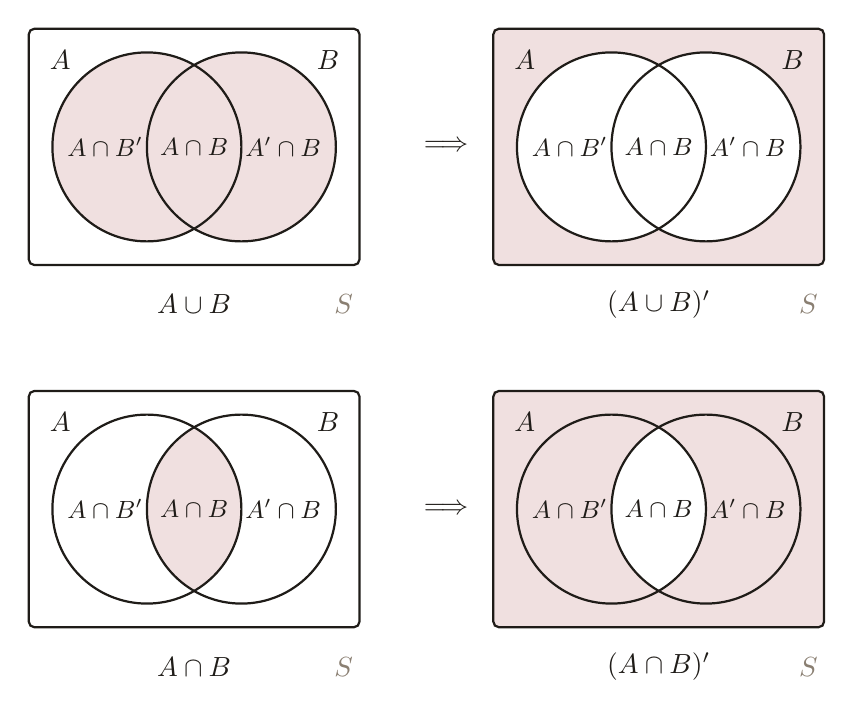
\begin{tikzpicture}[x=1cm, y=1cm, every node/.style={font=\normalsize}, accentfill/.style={fill=journalaccent, fill opacity=0.15}]

  %% Row 1, left: A cup B
  \begin{scope}[shift={(0,0)}]
    \begin{scope}
      \clip \panelbox;
      \path[accentfill] (0,0) circle (1.2) (1.2,0) circle (1.2);
    \end{scope}
    \twocircleframe
    \panelcaption{$A\cup B$}
    \spacelabel
    \node[journalink] at (3.8,0) {$\Longrightarrow$};
  \end{scope}

  %% Row 1, right: (A cup B)' = A' cap B'
  \begin{scope}[shift={(5.9,0)}]
    \begin{scope}[even odd rule]
      \clip \circA \panelbox;
      \begin{scope}[even odd rule]
        \clip \circB \panelbox;
        \path[accentfill] \panelbox;
      \end{scope}
    \end{scope}
    \twocircleframe
    \panelcaption{$(A\cup B)'$}
    \spacelabel
  \end{scope}

  %% Row 2, left: A cap B
  \begin{scope}[shift={(0,-4.6)}]
    \begin{scope}
      \clip \circA;
      \path[accentfill] \circB;
    \end{scope}
    \twocircleframe
    \panelcaption{$A\cap B$}
    \spacelabel
    \node[journalink] at (3.8,0) {$\Longrightarrow$};
  \end{scope}

  %% Row 2, right: (A cap B)' = A' cup B'
  \begin{scope}[shift={(5.9,-4.6)}]
    \begin{scope}[even odd rule]
      \clip \circA \panelbox;
      \path[accentfill] \panelbox;
    \end{scope}
    \begin{scope}[even odd rule]
      \clip \circB \panelbox;
      \path[accentfill] \circA;
    \end{scope}
    \twocircleframe
    \panelcaption{$(A\cap B)'$}
    \spacelabel
  \end{scope}

\end{tikzpicture}
\end{document}
